\documentclass[12pt]{article}
\usepackage[spanish,activeacute]{babel}
\usepackage{graphicx}
\usepackage{wrapfig}
\usepackage[utf8]{inputenc}
\usepackage[margin=3cm]{geometry}
\usepackage{hyperref} 

\begin{document}


\begin{picture}(18,4)
\put(140,-220){
\includegraphics[width=5cm,height=5cm]{espol.png}}
\end{picture}

\begin{center}


\textbf{{\Huge Escuela Superior Politécnica del Litoral}\\[7cm]
{\LARGE Lenguajes de Programación}}\\[3.5cm]

{\LARGE \textbf{Manual de Usuario}}\\[1.5cm]
{\large Charlie Medina \\Joseph Gallardo\\ Kevin Zambrano}\\[2cm]
Ingeniería en Ciencias Computacionales\\[1cm]
Guayaquil - \today
\end{center}



\title{\bfseries\Huge Sudoku\\ Manual de usuario}

\date{}



\begin{minipage}{0.55\textwidth}
\begingroup
\let\center\flushleft
\let\endcenter\endflushleft
\maketitle

\endgroup
\end{minipage}
\begin{minipage}{0.1\textwidth}
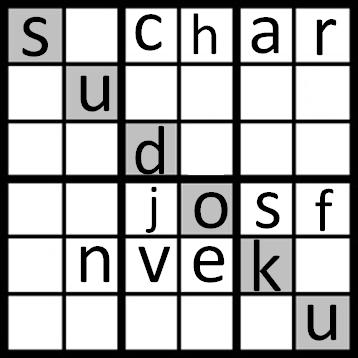
\includegraphics[height=6cm,width=8cm]{logo} 


\end{minipage}





\section{Introducción}

Sudoku es un pasatiempo que se publicó por primera vez a finales de la década de 1970 y se popularizó en Japón en 1986, dándose a conocer en el ámbito internacional en 2005 cuando numerosos periódicos empezaron a publicarlo en su sección de pasatiempos. El objetivo del sudoku es rellenar una cuadrícula de 9 x 9 celdas (81 casillas) dividida en subcuadrículas de 3 x 3 (también llamadas "cajas" o "regiones") con las cifras del 1 al 9 partiendo de algunos números ya dispuestos en algunas de las celdas, y lo característico del juego es llenar las casillas vacías con números que no se  repitan en una misma fila, columna o subcuadrícula. \\\\
\begin{center}
		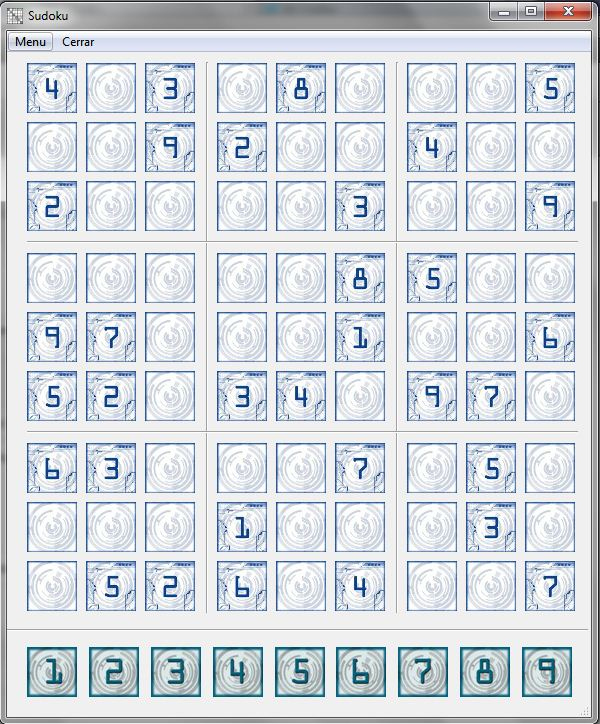
\includegraphics[height=9cm,width=7cm]{dificil.jpg}
	\end{center}
	
	




\section{Recorriendo Sudoku JCK}

	Nuestro Sudoku muestra en primera instacia la siguiente ventana:

	\begin{center}
		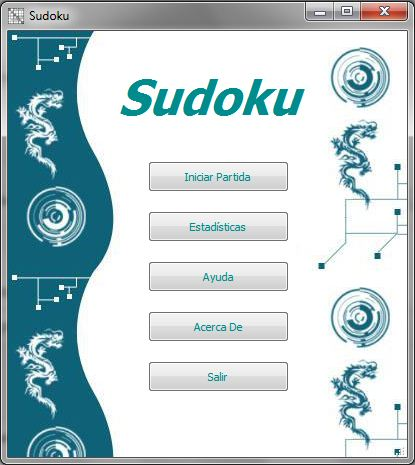
\includegraphics[height=6cm,width=8cm]{principal.jpg}
	\end{center}

	\subsection{Iniciar Partida}
		Esta opcion dará inicio a la partida correspondiente a jugar mostrando la siguiente venta que será la elección del respectivo nivel.

	\begin{center}
		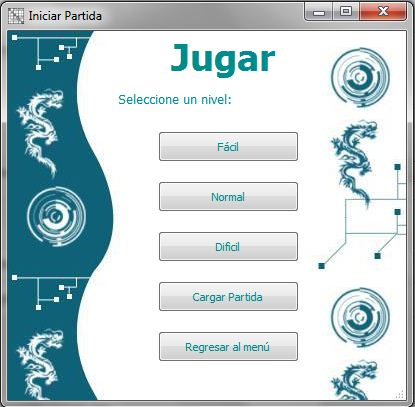
\includegraphics[height=5cm,width=4cm]{jugar.jpg}
	\end{center}


	\subsection{Estadísticas}
		Mostrará una ventana con los rankins de los mejores jugadores que hayan ganado una partida de sudoku.

	\begin{center}
		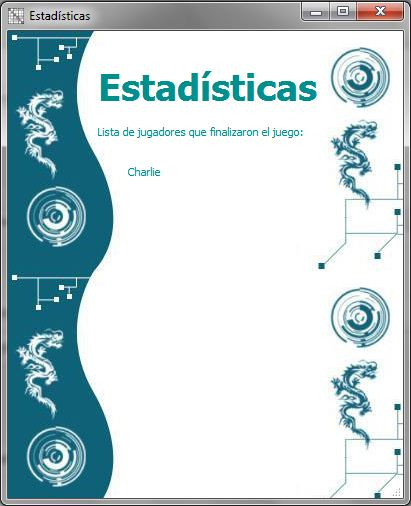
\includegraphics[height=5cm,width=4cm]{estadisticas.jpg}
	\end{center}

	\subsection{Ayuda}
		Se mostrará una ventana con una introduccion del juego y las reglas respectivas del mismo.

	\begin{center}
		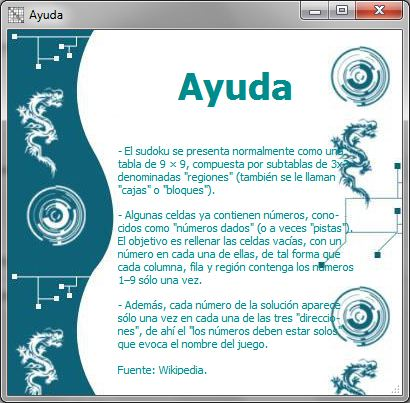
\includegraphics[height=5cm,width=4cm]{ayuda.jpg}
	\end{center}

	\subsection{Acerca De}
		Se mostrara una ventana con las referencias del juego y los nombres de sus desarrolladores.

	\begin{center}
		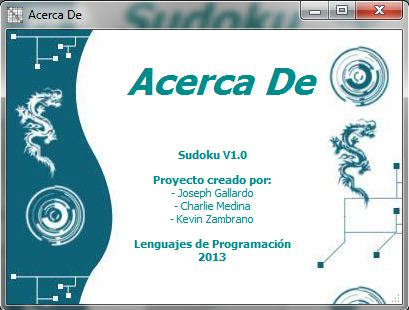
\includegraphics[height=5cm,width=4cm]{acercade.jpg}
	\end{center}

	\subsection{Salir}
		Mostrará una ventana solicitando la confirmación de salida al usuario.

\section{Recorriendo el Juego.}
	Al haber escogido la opción 'Iniciar Partida', la siguiente ventana de niveles se despliega:
		\begin{center}
			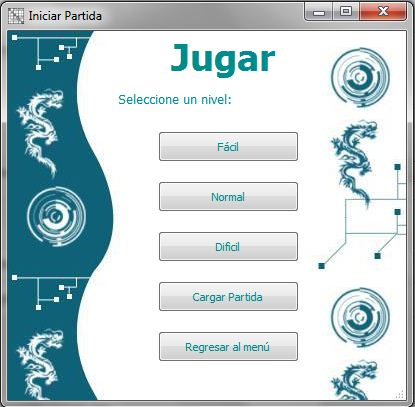
\includegraphics[height=5cm,width=7cm]{jugar.jpg}
		\end{center}
	La dificultad se basa en restar la cantidad de números al tablero, la cantidad de casillas blancas son:
		Facil   - 27 casillas vacias.

		\begin{center}
			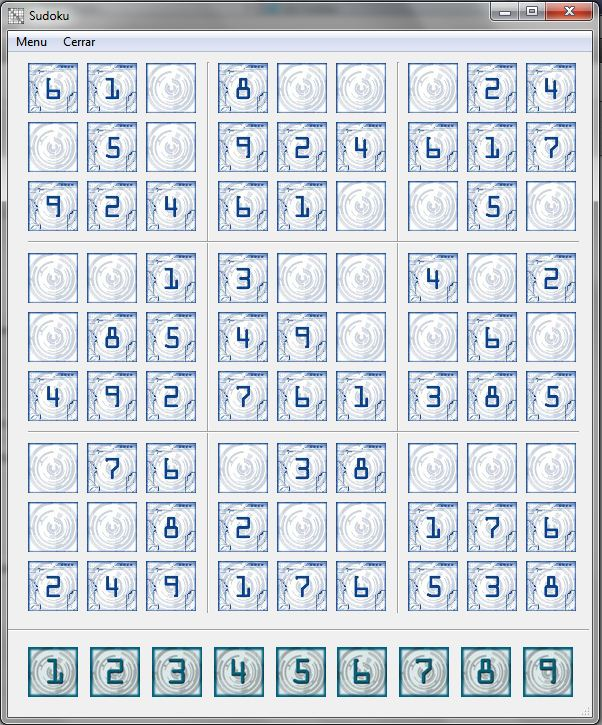
\includegraphics[height=5cm,width=4cm]{facil.jpg}
		\end{center}

		Medio - 41 casillas vacias.

		\begin{center}
			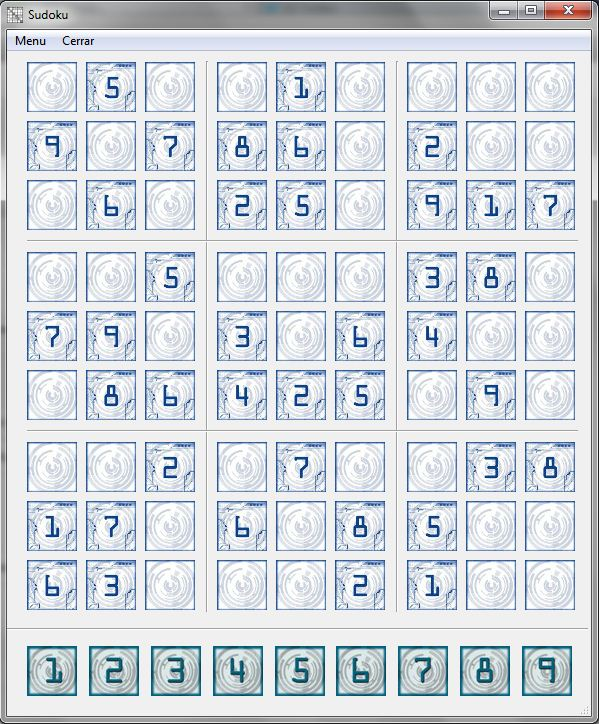
\includegraphics[height=5cm,width=4cm]{normal.jpg}
		\end{center}

		Dificil  - 48 casillas vacias.

		\begin{center}
			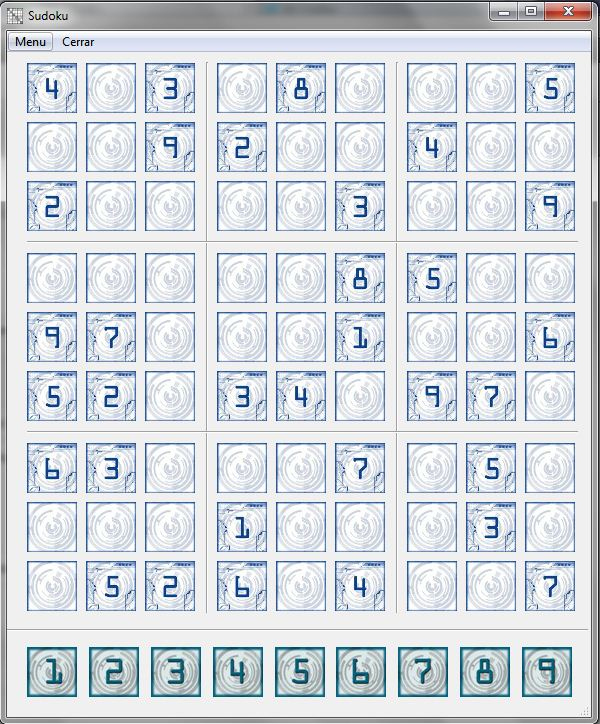
\includegraphics[height=5cm,width=4cm]{dificil.jpg}
		\end{center}

		Tambien se muestra la opcion 'Cargar Partida' la cual muestra una partida guardada previamente.	
		Una vez escogido el nivel, aparecerá la ventana del sudoku lista para ser jugada como se muestra en las figuras anteriores.

		
		
		



		


\end{document}